\section{Data Preparation}

\subsection{What was your data source (e.g., web scraping, corporate data, a standard machine learning data set, open data, etc.)?}

The dataset used in this study is sourced from open data published by the Government of Canada, on its Open Government Portal, an official government website. The use of open data from a reputable government source enhances transparency and allows for reproducibility in research.

\subsection{How good was the data quality?}



\subsection{What did you need to do to procure it?}

To procure the dataset, we downloaded the csv of the dataset and we ingested it using the pandas library.

\subsection{What tools or code did you need to use to prepare it for analysis?}

First, we segmented our analysis into three distinct categories: Chicken Meat, Hogs, and Wheat. The main libraries we used for our analysis were pandas, seaborn, numpy and statsmodels.api.Utilizing a dedicated helper function, we crafted time series plots for each category, with a focus on prices—a pivotal variable in our analysis. To ensure data completeness, we applied a boolean mask to handle null values. While exploring the data we recognized the historical prices of Newfoundland is very different from other provinces as you can see in Figure~\ref{fig:chicken_prices} so we decided to exclude Newfoundland from our analysis. We decided that it would be easiest to work with the data if all the prices were aggregated into a single response so we created a time series for each category where the mean prices for each category is the data and the datetime objects as the index.

\subsection{What challenges did you face?}

One notable hurdle emerged with certain features, like 'ref date', initially recorded as text, necessitating a round of feature engineering to render them immediately usable. The pricing dataset, with its varied units of measurement for a single commodity, introduced complexity, prompting us to carefully address this diversity during our analysis. The Wheat production dataset presented its own intricacies, featuring multiple entries for a given year. This intricacy made comparisons with other commodities a nuanced task. Meanwhile, the diverse data ranges of farm products posed a challenge in selecting the most pertinent ones for our analytical lens. The separation of price and production datasets added layers of complexity, urging us to integrate these disparate sources for a more comprehensive understanding. Addressing null values within the merged datasets became another crucial step in ensuring the integrity of our analysis.


\begin{figure}
    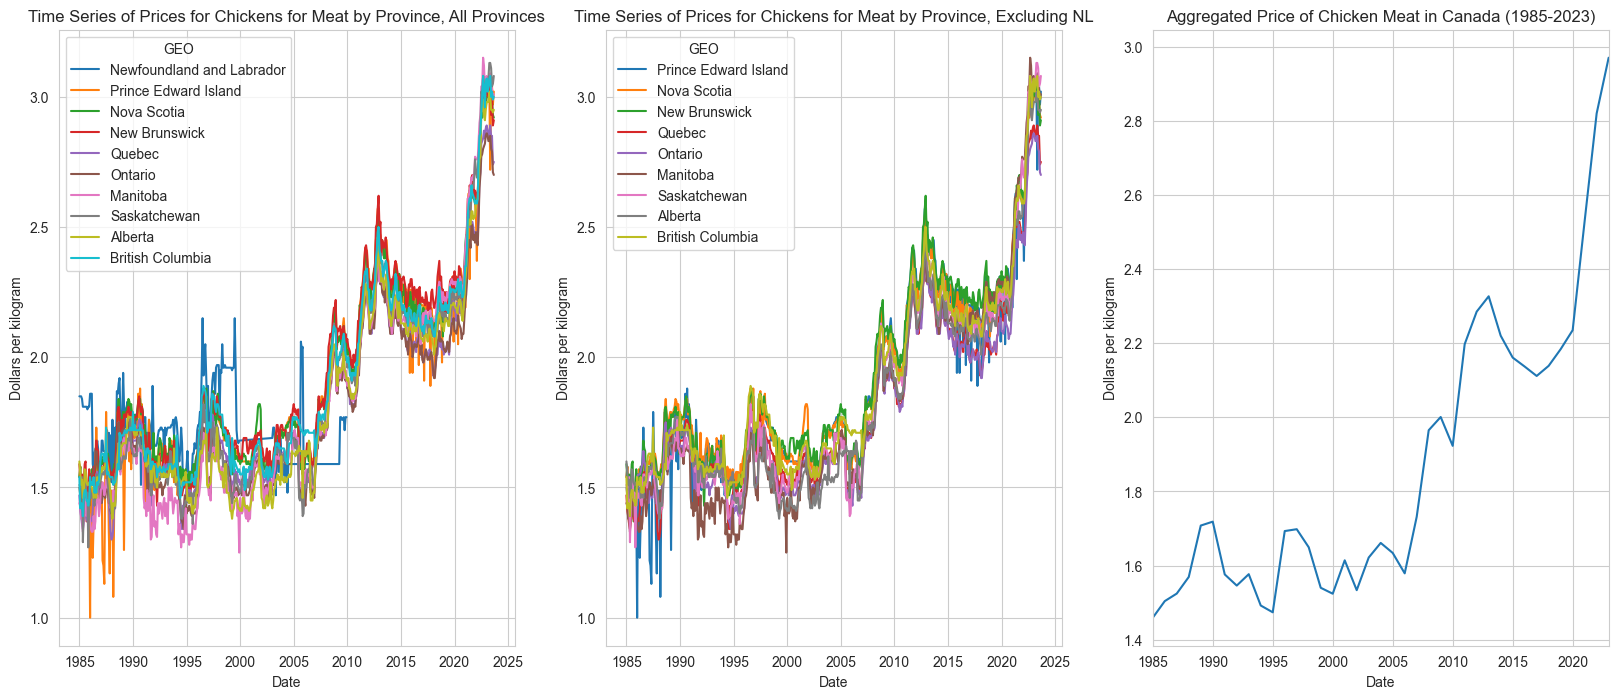
\includegraphics[width=\linewidth]{chicken_prices}
    \caption{This figure shows the raw data, and aggregated forms of chicken prices. MORE TEXT NEEDED?}
    \label{fig:chicken_prices}
\end{figure}


\begin{figure}
    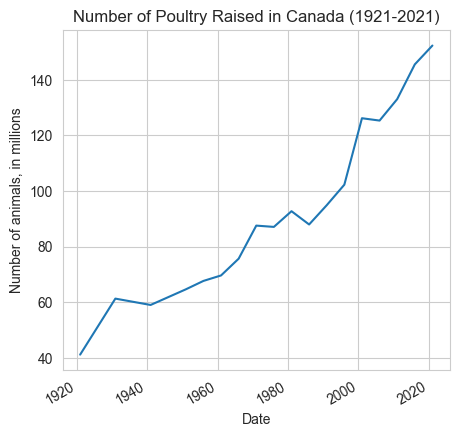
\includegraphics[width=\linewidth]{chicken_production_time_series}
    \caption{This figure shows the number of chickens counted on chicken farms in Canada between 1921-2021.}
    \label{fig:chicken_production}
\end{figure}